\chapter{Mutation, Migration, and Genetic Drift}

So far in this course we've focused on single, isolated populations,
and we've imagined that there isn't any mutation. We've also
completely ignored the ultimate source of all genetic
variation{\dash}mutation.\footnote{Well, that's not quite true. We
  talked about multiple populations when we talked about the Wahlund
  effect and Wright's $F_{ST}$, but we didn't talk explicitly about
  any of the evolutionary processes associated with multiple
  populations.} We're now going to study what happens when we consider
multiple populations simultaneously and when we allow mutation to
happen. Let's consider mutation first, because it's the easiest to
understand.

\section*{Drift and mutation}\index{genetic drift!mutation}

Remember that in the absence of mutation
\begin{equation}
f_{t+1} = \left(\frac{1}{2N}\right) +
          \left(1 - \frac{1}{2N}\right)f_t \quad \label{eq:f} ,
\end{equation}
One way of modeling mutation is to assume that every time a mutation
occurs it introduces a new allele into the population. This model is
referred to as the {\it infinite alleles model}, because it implicitly
assumes that there is potentially an infinite number of
alleles.\index{mutation!infinite alleles model} Under this model we
need to make only one simple modification to equation (\ref{eq:f}). We
have to multiply the expression on the right by the probability that
neither allele mutated:
\begin{equation}
f_{t+1} = \left(\left(\frac{1}{2N}\right) +
          \left(1 - \frac{1}{2N}\right)f_t\right)(1-\mu)^2 \quad
\label{eq:f-mu} ,
\end{equation}
where $\mu$ is the mutation rate, i.e., the probability that an allele
in an offspring is different from the allele it was derived from in a
parent. In writing down this expression, the reason this is referred
to as an infinite alleles model becomes apparent: we are assuming that
every time a mutation occurs it produces a new allele. The only way in
which two alleles can be identical is if neither
mutated.\footnote{Notice that we're also playing a little fast and
  loose with definitions here, since I've just described this in terms
  of identity by type when what the equation is written in terms of
  identity by descent. Can you see why it is that I can get away with
  this?}

So where do we go from here? Well, if you think about it, mutation is
always introducing new alleles that, by definition, are different from
any of the alleles currently in the population. It stands to reason,
therefore, that we'll never be in a situation where all of the alleles
in a population are identical by descent as they would be in the
absence of mutation. In other words we expect there to be an
equilibrium between loss of diversity through genetic drift and the
introduction of diversity through mutation.\footnote{Technically what
  the population reaches is not an equilibrium. It reaches a
  stationary distribution. At any point in time there is some
  probability that the population has a particular allele
  frequency. After long enough the probability distribution stops
  changing. That's when the population is at its stationary
  distribution. We often say that it's ``reached stationarity.'' This
  is an example of a place where the inbreeding analogy breaks down a
  little.}\index{genetic drift!mutation, stationary distribution} From the
definition of an equilibrium,
\begin{eqnarray*}
\hat f &=& \left(\left(\frac{1}{2N}\right) +
          \left(1 - \frac{1}{2N}\right)\hat f\right)(1-\mu)^2 \\
\hat f\left(1 -
\left(1 - \frac{1}{2N}\right)(1-\mu)^2\right)
       &=& \left(\frac{1}{2N}\right)(1-\mu)^2 \\
\hat f &=& \frac{\left(\frac{1}{2N}\right)(1-\mu)^2}
           {1 -\left(1 - \frac{1}{2N}\right)(1-\mu)^2} \\
       &\approx& \frac{1 - 2\mu}
           {2N\left(1 - \left(1 - \frac{1}{2N}\right)(1-2\mu)\right)} \\
       &=& \frac{1 - 2\mu}
           {2N\left(1 - 1 + \frac{1}{2N} + 2\mu -
            \frac{2\mu}{2N}\right)} \\
       &=& \frac{1 - 2\mu}{1 + 4N\mu - 2\mu} \\
       &\approx& \frac{1}{4N\mu + 1}
\end{eqnarray*}

Since $f$ is the probability that two alleles chosen at random are
identical by descent within our population, $1-f$ is the probability
that two alleles chosen at random are {\it not\/} identical by descent
in our population. So $1-f = 4N\mu/(4N\mu + 1)$ is a reasonable
measure of the genetic diversity within the population. Notice that as
$N$ increases, the genetic diversity maintained in the population also
increases. This shouldn't be too surprising. The rate at which
diversity is lost declines as population size increases so larger
populations should retain more diversity than small
ones.\footnote{Remember that if we're dealing with a non-ideal
population, as we always are, you'll need to substitute $N_e$ for $N$
in this equation and others like it.}

\subsection*{A two-allele model with recurrent mutation}\index{genetic drift!mutation, recurrent}

There's another way of looking at the interaction between drift and
mutation. Suppose we have a set of populations with two alleles, $A_1$
and $A_2$. Suppose further that the rate of mutation from $A_1$ to
$A_2$ is equal to the rate of mutation from $A_2$ to
$A_1$.\footnote{We don't have to make this assumption, but relaxing it
makes an already fairly complicated scenario even more complicated. If
you're really interested, ask me about it.} Call that rate $\mu$. In
the absence of mutation a fraction $p_0$ of the populations would fix
on $A_1$ and the rest would fix on $A_2$, where $p_0$ is the original
frequency of $A_1$. With recurrent mutation, no population will ever
be permanently fixed for one allele or the other. Instead we see the
following:\index{genetic drift!mutation, stationary distribtuion}

\begin{center}
\resizebox{!}{8cm}{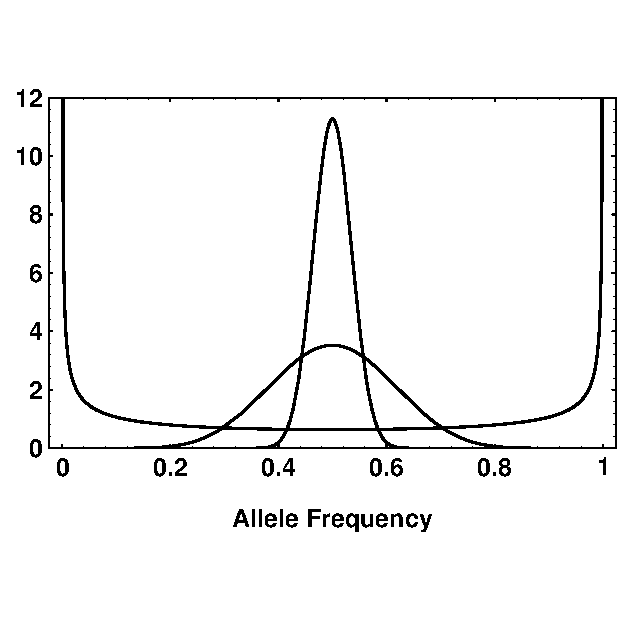
\includegraphics{mutation.eps}}
\end{center}

When $4N\mu < 1$ the stationary distribution of allele frequencies is
bowl-shaped, i.e, most populations have allele frequencies near 0 or
1. When $4N\mu > 1$, the stationary distribution of allele frequencies
is hump-shaped, i.e., most populations have allele frequencies near
0.5. In other words if the population is ``small,'' drift dominates
the distribution of allele frequencies and causes populations to
become differentiated. If the population is ``large,'' mutation
dominates and keeps the allele frequencies in the different
populations similar to one another. That's what we mean when we say
that a population is ``large'' or ``small''. A population is ``large''
if evolutionary processes other than drift have a predominant
influence on the outcom. It's ``small'' if drift has a predominant
role on the outcome.\index{genetic drift!population size}

A population is large with respect to the drift-mutation process if
$4N\mu > 1$, and it is small if $4N\mu < 1$. Notice that calling a
population large or small is really just a convenient shorthand. There
isn't much of a difference between the allele frequency distributions
when $4N\mu = 0.9$ and when $4N\mu = 1.1$. Notice also that because
mutation is typically rare, on the order of $10^{-5}$ or less per
locus per generation for a protein-coding gene and on the order of
$10^{-3}$ or less per locus for a microsatellite, a population must be
pretty large ($> 25,000$ or $>250$) to be considered large with
respect to the drift-migration process. Notice also that whether the
population is ``large'' or ``small'' will depend on the loci that
you're studying.

\section*{Drift and migration}\index{genetic drift!migration}

I just pointed out that if populations are isolated from one another
they will tend to diverge from one another as a result of genetic
drift. Recurrent mutation, which ``pushes'' all populations towards
the same allele frequency, is one way in which that tendency can be
opposed. If populations are not isolated, but exchange migrants with
one another, then migration will also oppose the tendency for
populations to become different from one another. It should be obvious
that there will be a tradeoff similar to the one with mutation: the
larger the populations, the less the tendency for them to diverge from
one another and, therefore, the more migration will tend to make them
similar. To explore how drift and migration interact we can use an
approach exactly analogous to what we used for mutation.

The model of migration we'll consider is an extremely oversimplified
one. It imagines that every allele brought into a population is
different from any of the resident alleles.\footnote{Sounds a lot like
  the infinite alleles model of mutation, doesn't it? Just you
  wait. The parallel gets even more striking.} It also imagines that
all populations receive the same fraction of migrants. Because any
immigrant allele is different, by assumption, from any resident allele
we don't even have to keep track of how far apart populations are from
one another, since populations close by will be no more similar to one
another than populations far apart. This is Wright's island model of
migration. Given these assumptions, we can write the following:
\begin{equation}
f_{t+1} = \left(\left(\frac{1}{2N}\right) +
          \left(1 - \frac{1}{2N}\right)f_t\right)(1-m)^2 \quad
\label{eq:f-m} .
\end{equation}

That might look fairly familiar. In fact, it's identical to equation
(\ref{eq:f-mu}) except that there's an $m$ in (\ref{eq:f-m}) instead
of a $\mu$. $m$ is the migration rate, the fraction of individuals in
a population that is composed of immigrants. More precisely, $m$ is
the {\it backward\/} migration rate.\index{migration rate!backward}
It's the probability that a randomly chosen individual in this
generation {\it came from\/} a population different from the one in
which it is currently found in the preceding generation. Normally we'd
think about the {\it forward\/} migration rate,\index{migration rate!forward}  i.e., the probability
that a randomly chosen individual with {\it go to\/} a different
population in the next generation, but backwards migration rates turn
out to be more convenient to work with in most population genetic
models.\footnote{I warned you weeks ago that population geneticists
  tend to think backwards.}

It shouldn't surprise you that if equations (\ref{eq:f-mu}) and
(\ref{eq:f-m}) are so similar the equilibrium $f$ under drift and
migration is
\[
\hat f \approx \frac{1}{4Nm + 1}
\]
In fact, the two allele analog to the mutation model I presented
earlier turns out to be pretty similar, too.

\begin{itemize}

\item If $2Nm > 1$, the stationary distribution of allele frequencies
is hump-shaped, i.e., the populations tend not to diverge from one
another.\footnote{You read that right it's $2Nm$ not $4Nm$ as you
might have expected from the mutation model. If you're {\it really\/}
interested why there's a difference, I can show you. But the
explanation isn't simple.}

\item If $2Nm < 1$, the stationary distribution of allele frequencies
is bowl-shaped, i.e., the populations tend to diverge from one another.

\end{itemize}

Now there's a consequence of these relationships that's both
surprising and odd. $N$ is the population size. $m$ is the fraction of
individuals in the population that are immigrants. So $Nm$ is the {\it
  number\/} of individuals in the population that are new immigrants
in any generation. That means that if populations receive more than
one new immigrant every other generation, on average, they'll tend not
to diverge in allele frequency from one another.\footnote{In the sense
  that the stationary distribution of allele frequencies is
  hump-shaped.} It doesn't make any difference if the populations have
a million individuals apiece or ten. One new immigrant every other
generation is enough to keep them from diverging.

With a little more reflection, this result is less surprising than it
initially seems. After all in populations of a million individuals,
drift will be operating very slowly, so it doesn't take a large
proportion of immigrants to keep populations from
diverging.\footnote{And one immigrant every other generation
  corresponds to a backwards migration rate of only $5\times
  10^{-7}$.} In populations with only ten individuals, drift will be
operating much more quickly, so it takes a large proportion of
immigrants to keep populations from diverging.\footnote{And one
  immigrant every other generation corresponds to a backwards
  migration rate of $5 \times 10^{-2}$.}

